\chapter{The \corrybold Framework}
\label{ch:framework}

\corry  is based on a collection of modules read from a configuration file and an event loop which sequentially processes data from all detectors assigned to one event.
In each loop iteration, all modules are executed in the linear order they appear in the configuration file and have access to all data created by previous modules.
At the end of the loop iteration, the data cache is cleared and the framework continues with processing the next iteration.
This chapter provides basic information about the different components of the framework, its executable as well as the available configuration parameters that are processed on a global level.

\section{The \texttt{corry} Executable}
\label{sec:executable}
The \corry executable \command{corry} functions as the interface between the user and the framework.
It is primarily used to provide the main configuration file, but also allows options from the main configuration file to be added or overwritten.
This is useful for quick testing as well as for batch processing of many runs to be reconstructed.

The executable handles the following arguments:
\begin{itemize}
\item \texttt{-c <file>}: Specifies the configuration file to be used for the reconstruction, relative to the current directory.
This is the only \textbf{required} argument and the program will fail to start if this argument is not given.
\item \texttt{-l <file>}: Specify an additional location, such as a file to forward log output into. This is used as an additional destination alongside the standard output and the location specified in the framework parameters described in Section~\ref{sec:framework_parameters}.
\item \texttt{-v <level>}: Sets the global log verbosity level, overwriting the value specified in the configuration file described in Section~\ref{sec:framework_parameters}.
Possible values are \texttt{FATAL}, \texttt{STATUS}, \texttt{ERROR}, \texttt{WARNING}, \texttt{INFO} and \texttt{DEBUG}, where all options are case-insensitive.
The module specific logging level introduced in Section~\ref{sec:logging_verbosity} is not overwritten.
\item \texttt{-o <option>}: Passes extra framework or module options that adds to and/or overwrites those in the main configuration file.
This argument may be specified multiple times to add multiple options.
Options are specified as key-value pairs in the same syntax as used in the configuration files described in Chapter~\ref{ch:configuration_files}, but the key is extended to include a reference to a configuration section or instantiation in shorthand notation.
There are three types of keys that can be specified:
\begin{itemize}
    \item Keys to set \textbf{framework parameters}: These have to be provided in exactly the same way as they would be in the main configuration file (a section does not need to be specified). An example to overwrite the standard output directory would be \texttt{corry -c <file> -o output\_directory="run123456"}.
    \item Keys for \textbf{module configurations}: These are specified by adding a dot (\texttt{.}) between the module and the key as it would be given in the configuration file (thus \textit{module}.\textit{key}). An example to overwrite the number of hits required for accepting a track candidate would be \command{corry -c <file> -o Tracking4D.min_hits_on_track=5}.
    \item Keys to specify values for a particular \textbf{module instantiation}: The identifier of the instantiation and the name of the key are split by a dot (\texttt{.}), in the same way as for keys for module configurations (thus \textit{identifier}.\textit{key}). The unique identifier for a module can contain one or more colons (\texttt{:}) to distinguish between various instantiations of the same module. The exact name of an identifier depends on the name of the detector. An example to change the neighbor pixel search radius of the clustering algorithm for a particular instantiation of the detector named \textit{my\_dut} could be \command{corry -c <file> -o Clustering4D:my_dut.neighbor_radius_row=2}.
\end{itemize}
Note that only the single argument directly following the \texttt{-o} is interpreted as the option. If there is whitespace in the key-value pair this should be properly enclosed in quotation marks to ensure that the argument is parsed correctly.
\item \texttt{-g <option>}: Passes extra detector options that are added to and/or overwritten in the detector configuration file.
This argument can be specified multiple times to add multiple options.
The options are parsed in the same way as described above for module options, but only one type of key can be specified to overwrite an option for a single detector.
These are specified by adding a dot (\texttt{.}) between the detector and the key as it would be given in the detector configuration file (thus \textit{detector}.\textit{key}). An example to change the orientation of a particular detector named \texttt{detector1} would be \texttt{corry -c <file> -g detector1.orientation=0deg,0deg,45deg}.
\end{itemize}

No direct interaction with the framework is possible during the reconstruction. Signals can be sent using keyboard shortcuts to terminate the run, either gracefully or with force. The executable understands the following signals:
\begin{itemize}
\item SIGINT (\texttt{CTRL+C}): Request a graceful shutdown of the reconstruction. This means the event currently being processed is finished, while all other events requested in the configuration file are ignored. After finishing the event, the finalization stage is executed for every module to ensure all modules finish properly.
\item SIGTERM: Same as SIGINT, request a graceful shutdown of the reconstruction. This signal is emitted e.g.\ by the \command{kill} command or by cluster computing schedulers to ask for a termination of the job.
\item SIGQUIT (\texttt{CTRL+\textbackslash}): Forcefully terminates the framework. It is not recommended to use this signal as it will normally lead to the loss of all generated data. This signal should only be used when graceful termination is not possible.
\end{itemize}

\section{The Clipboard}

The clipboard is the framework infrastructure for temporarily storing information during the event processing.
Every module can access the clipboard to both read and write information.
Collections or individual elements on the clipboard are accessed via their data type, and an optional key can be used in addition to identify them with a certain detector by its name.

The clipboard consists of three parts: the event, a temporary data storage, and a persistent storage space.

\subsection{The Event}

The event is the central element storing meta-information about the data currently processed.
This includes the time frame (or data slice) within which all data are located as well as trigger numbers associated with these data.
New data to be added are always compared to the event on the clipboard to determine whether they should be discarded, included, or buffered for later use.
A detailed description of the event building process is provided in Chapter~\ref{ch:events}.

\subsection{Temporary Data Storage}
The temporary data storage is only available during the processing of each individual event.
It is automatically cleared at the end of the event processing and has to be populated with new data in the new event to be processed.

The temporary storage acts as the main data structure to communicate information between different modules and can hold multiple collections of \corry objects such as pixel hits, clusters, or tracks.
In order to be able to flexibly store different data types on the clipboard, the access methods for the temporary data storage are implemented as templates, and vectors of any data type deriving from \parameter{corry::Object} can be stored and retrieved.

\subsection{Persistent Storage}
The persistent storage is not cleared at the end of processing each event and can therefore be used to store information across multiple events or even until the end of the run.
This allows for example to accumulate tracks over a full run for an alignment procedure executed at the very end of the run.

The persistent storage element has the same data access methods as the temporary event storage. In addition, a helper function allows to provide raw pointers to data stored on the temporary storage element in order to directly copy over the relevant data to persistent storage.

\begin{warning}
    The persistent clipboard storage does not automatically resolve object history. This means in order to access for example the clusters referenced in a track at the end of the run, both the track and the relevant cluster objects have to be copied to the persistent storage.
    Not copying the clusters will lead to missing data and unavailable references.
\end{warning}


\section{Global Framework Parameters}
\label{sec:framework_parameters}
The \corry framework provides a set of global parameters that control and alter its behavior. These parameters are inherited by all modules.
The currently available global parameters are:

\begin{itemize}
\item \parameter{detectors_file}: Location of the file describing the detector configuration described in Section~\ref{sec:detector_config}.
The only \textit{required} global parameter as the framework will fail to start if it is not specified.
This parameter can take multiple paths; all provided files will be combined into one geometry description of the setup.
\item \parameter{detectors_file_updated}: Location of the file that the (potentially) updated detector configuration should be written into. If this file does not already exist, it will be created. If the same file is given as for \parameter{detectors_file}, the file is overwritten. If no file is specified using this parameter then the updated geometry is not written to file.
\item \parameter{histogram_file}: Location of the file where the ROOT output histograms of all modules will be written to. The file extension \texttt{.root} will be appended if not present. Directories within the ROOT file will be created automatically for all modules.
\item \parameter{number_of_events}: Determines the total number of events the framework will process, where negative numbers allow for the processing of all data available.
After reaching the specified number of events, the reconstruction is stopped.
Defaults to $-1$.
\item \parameter{number_of_tracks}: Determines the total number of tracks the framework should reconstruct, where negative numbers indicate that there is no limit on the number of reconstructed tracks.
After reaching the specified number of events, the reconstruction is stopped.
Defaults to $-1$.
\item \parameter{run_time}: Determines the wall-clock time of data acquisition the framework should reconstruct up until. Negative numbers indicate that there is no limit on the time slice to reconstruct.
Defaults to $-1$.
\item \parameter{log_level}: Specifies the lowest log level that should be reported.
+Possible values are \texttt{FATAL}, \texttt{STATUS}, \texttt{ERROR}, \texttt{WARNING}, \texttt{INFO}, and \texttt{DEBUG}, where all options are case-insensitive.
Defaults to the \texttt{INFO} level.
More details and information about the log levels, including how to change them for a particular module, can be found in Section~\ref{sec:logging_verbosity}.
Can be overwritten by the \texttt{-v} parameter on the command line (see Section~\ref{sec:executable}).
\item \parameter{log_format}: Determines the log message format to be displayed.
Possible options are \texttt{SHORT}, \texttt{DEFAULT}, and \texttt{LONG}, where all options are case-insensitive.
More information can be found in Section~\ref{sec:logging_verbosity}.
\item \parameter{log_file}: File where the log output will be written, in addition to the standard printing (usually the terminal).
Another (additional) location to write to can be specified on the command line using the \texttt{-l} parameter (see Section~\ref{sec:executable}).
\item \parameter{library_directories}: Additional directories to search in for module libraries, before searching the default paths.
\item \parameter{output_directory}: Directory to write all output files into.
Subdirectories are created automatically for all module instantiations.
This directory will also contain the \parameter{histogram_file} specified via the parameter described above.
Defaults to the current working directory with the subdirectory \dir{output/} attached.
\item \parameter{purge_output_directory}: Decides whether the content of an already existing output directory is deleted before a new run starts. Defaults to \texttt{false}, i.e. files are kept but will be overwritten by new files created by the framework.
\item \parameter{deny_overwrite}: Forces the framework to abort the run and throw an exception when attempting to overwrite an existing file. Defaults to \texttt{false}, i.e. files are overwritten when requested. This setting is inherited by all modules, but can be overwritten in the configuration section of each of the modules.
\end{itemize}

\section{Modules and the Module Manager}
\label{sec:module_manager}
\corry is a modular framework and one of the core ideas is to partition functionality into independent modules that can be inserted or removed as required.
These modules are located in the subdirectory \dir{src/modules/} of the repository, with the name of the directory as the unique name of the module.
The suggested naming scheme is CamelCase, thus an example module name would be \module{OnlineMonitor}.
Any \emph{specifying} part of a module name should precede the \emph{functional} part of the name, e.g.\ \module{EventLoaderCLICpix2} rather than \module{CLICpix2EventLoader}.
There are three different kinds of modules that can be defined:
\begin{itemize}
    \item \textbf{Global}: Modules for which a single instance runs, irrespective of the number of detectors.
    \item \textbf{Detector}: Modules that are concerned with only a single detector at a time.
    These are then replicated for all required detectors.
    \item \textbf{DUT}: Similar to the Detector modules, these modules run for a single detector.
    However, they are only replicated if the respective detector is marked as device-under-test (DUT).
\end{itemize}
The type of module determines the constructor used, the internal unique name, and the supported configuration parameters.
For more details about the instantiation logic for the different types of modules, see Section~\ref{sec:module_instantiation}.

Furthermore, detector modules can be restricted to certain types of detectors.
This allows the framework to automatically determine for which of the given detectors the respective module should be instantiated.
For example, the \module{EventLoaderCLICpix2} module will only be instantiated for detectors with the correct type \parameter{CLICpix2} without any additional configuration effort required by the user.
This procedure is described in more detail in Section~\ref{sec:module_files}.

\subsection{Module Status Codes}

The \command{run()} function of each module returns a status code to the module manager to indicate the status of the module.
These codes can be used to e.g. request the end of the current run or to signal problems in data processing.
The following status codes are currently supported:

\begin{description}
    \item{\command{Success}}: Indicates that the module successfully finished processing all data. The framework continues with the next module.
    \item{\command{NoData}}: Indicates that the respective module did not find any data to process. The framework continues with the next module.
    \item{\command{DeadTime}}: Indicates that the detector handled by the respective module is currently in data acquisition dead time. The framework skips all remaining modules for this event and continues with the subsequent event. By employing this method, measurements such as efficiency are not affected by known inefficiencies during detector dead times.
    \item{\command{EndRun}}: Allows the module to request a premature end of the run. This can e.g.\ be used by alignment modules to stop the run after they have accumulated enough tracks for the alignment procedure. The framework executes all remaining modules for the current event and then enters the finalization stage.
    \item{\command{Failure}}: Indicates that there was a severe problem when processing data in the respective module. The framework skips all remaining modules for this event and enters the finalization stage.
\end{description}

\subsection{Execution Order}

Modules are executed in the order in which they appear in the configuration file; the sequence is repeated for every time frame or event.
If one module in the chain raises e.g.\ a \command{DeadTime} status, the processing of the next event is begun without executing the remaining modules for the current event.

The execution order is of special importance in the event building process, since the first module will always have to define the event while subsequent event loader modules will have to adhere to the time frame defined by the first module.
A complete description of the event building process is provided in Chapter~\ref{ch:events}.

This behavior should also be taken into account when choosing the order of modules in the configuration file, since e.g.\ data from detectors catered by subsequent event loaders is not processed and hit maps are not updated if an earlier module requested to skip the rest of the module chain.

\subsection{Module instantiation}
\label{sec:module_instantiation}
Modules are dynamically loaded and instantiated by the Module Manager.
They are constructed, initialized, executed, and finalized in the linear order in which they are defined in the configuration file. For this reason, the configuration file should follow the order of the real process.
For each section in the main configuration file (see Chapter~\ref{ch:configuration_files} for more details), a corresponding library is searched for which contains the module (the exception being the global framework section).
Module libraries are always named following the scheme \textbf{libCorryvreckanModule\texttt{ModuleName}}, reflecting the \texttt{ModuleName} configured via CMake.
The module search order is as follows:
\begin{enumerate}
\item Modules already loaded from an earlier section header
\item All directories in the global configuration parameter \parameter{library_directories} in the provided order, if this parameter exists.
\item The internal library paths of the executable, which should automatically point to the libraries that are built and installed together with the executable.
These library paths are stored in \dir{RPATH} on Linux, see the next point for more information.
\item The other standard locations to search for libraries depending on the operating system.
Details about the procedure Linux follows can be found in~\cite{linuxld}.
\end{enumerate}

If the loading of the module library is successful, the module is checked to determine if it is a global, detector, or DUT module.
A single module may be called multiple times in the configuration with overlapping requirements (such as a module that runs on all detectors of a given type, followed by the same module but with different parameters for one specific detector, also of this type). Hence the Module Manager must establish which instantiations to keep and which to discard.
The instantiation logic determines a unique name and priority for every instantiation. Internally these are handled as numerical values, where a lower number indicates a higher priority.
The name and priority for the instantiation are determined differently for the two types of modules:
\begin{itemize}
\item \textbf{Global}: Name of the module, the priority is always \emph{high}.
\item \textbf{Detector/DUT}: Combination of the name of the module and the name of detector this module is executed for.
If the name of the detector is specified directly by the \parameter{name} parameter, the priority is \emph{high}.
If the detector is only matched by the \parameter{type} parameter, the priority is \emph{medium}.
If the \parameter{name} and \parameter{type} are both unspecified and the module is instantiated for all detectors, the priority is \emph{low}.
\end{itemize}
In the end, only a single instance for every unique name is allowed.
If there are multiple instantiations with the same unique name, the instantiation with the highest priority is kept.
If multiple instantiations with the same unique name and the same priority exist, an exception is raised.

\section{Logging and Verbosity Levels}
\label{sec:logging_verbosity}
\corry is designed to identify mistakes and implementation errors as early as possible and to provide the user with clear indications of the location and cause the problem.
The amount of feedback can be controlled using different log levels, which are inclusive, i.e.\ lower levels also include messages from all higher levels.
The global log level can be set using the global parameter \parameter{log_level}.
The log level can be overridden for a specific module by adding the \parameter{log_level} parameter to the respective configuration section.
The following log levels are supported:
\begin{itemize}
\item \textbf{FATAL}: Indicates a fatal error that will lead to the direct termination of the application.
Typically only emitted in the main executable after catching exceptions, as they are the preferred way of fatal error handling.
An example of a fatal error is an invalid value for an existing configuration parameter.
\item \textbf{STATUS}: Important information about the status of the reconstruction.
Is only used for messages that have to be logged in every run, such as initial information on the module loading, opened data files, and the current progress of the run.
\item \textbf{ERROR}: Severe error that should not occur during a normal, well-configured reconstruction.
Frequently leads to a fatal error and can be used to provide extra information that may help in finding the problem. For example, it is used to indicate the reason a dynamic library cannot be loaded.
\item \textbf{WARNING}: Indicate conditions that should not occur normally and possibly lead to unexpected results.
The framework will however continue without problems after a warning.
A warning is, for example, issued to indicate that a calibration file for a certain detector cannot be found and that the reconstruction is therefore performed with uncalibrated data.
\item \textbf{INFO}: Information messages about the reconstruction process.
Contains summaries of the reconstruction details for every event and for the overall run.
This should typically produce at maximum one line of output per event and module.
\item \textbf{DEBUG}: In-depth details about the progress of the reconstruction, such as information on every cluster formed or on track fitting results.
Produces large volumes of output per event and should therefore only be used for debugging the reconstruction process.
\item \textbf{TRACE}: Messages to trace what the framework or a module is currently doing.
Unlike the \textbf{DEBUG} level, it does not contain any direct information about the physics but rather indicates which part of the module or framework is currently running.
Mostly used for software debugging or determining performance bottlenecks in the reconstruction.
\end{itemize}

\begin{warning}
    It is not recommended to set the \parameter{log_level} higher than \textbf{WARNING} in a typical reconstruction as important messages may be missed.
    Setting too low logging levels should also be avoided since printing many log messages will significantly slow down the reconstruction.
\end{warning}

The logging system supports several formats for displaying the log messages.
The following formats are supported via the global parameter \parameter{log_format} or the individual module parameter with the same name:
\begin{itemize}
\item \textbf{SHORT}: Displays the data in a short form.
Includes only the first character of the log level followed by the configuration section header and the message.
\item \textbf{DEFAULT}: The default format.
Displays the system time, log level, section header, and the message itself.
\item \textbf{LONG}: Detailed logging format.
Displays all of the above but also indicates the source code file and line where the log message was produced.
This can help when debugging modules.
\end{itemize}

\section{Coordinate Systems}
\label{sec:coordinate_systems}

Local coordinate systems for each detector and a global frame of reference for the full setup are defined.
The global coordinate system is chosen as a right-handed Cartesian system, and the rotations of individual devices are performed around the geometrical center of their sensor.
Here, the beam direction defines the positive z-axis at the origin of the x-y-plane.
The origin along the z-axis is fixed by the placement of the detectors in the geometry of the setup.

There are several kinds of detectors with different local coordinate system, e.g., Cartesian coordinate for pixel detector and polar coordinate for some specific strip detectors. For this reason, the \textsl{Detector} class is designed as an interface, the detector with a specific coordinate system will be generated according to the parameter in the detector configuration file. In the current version, the Cartesian coordinate is the only available one.

For the local Cartesian coordinate system, it is right-handed with the x- and y-axes defining the sensor plane.  The origin of this coordinate system is the center of the lower left pixel in the grid, i.e.\ the pixel with indices (0,0).  This simplifies calculations in the local coordinate system as all positions can either be stated in absolute numbers or in fractions of the pixel pitch.

\subsection{Coordinate system for curved sensors}
\label{ssec:bentdetectors}

A coordinate system redefinition is needed in order to analyze data from curved sensors. A new ''\texttt{cartesian-bent}`` coordinate system is introduced. The local and global coordinate systems defined in \ref{sec:coordinate_systems} are not affected.

An idealized cylindrical geometry is chosen for transformations involving the new coordinate system. Only one bending direction is allowed at a time.

The bending was implemented for rectangular pixels, with some caveats for bending along rows or columns (see Fig.~\ref{fig:bent_coord_syst}). 


\begin{figure}[!htp]
\centering
  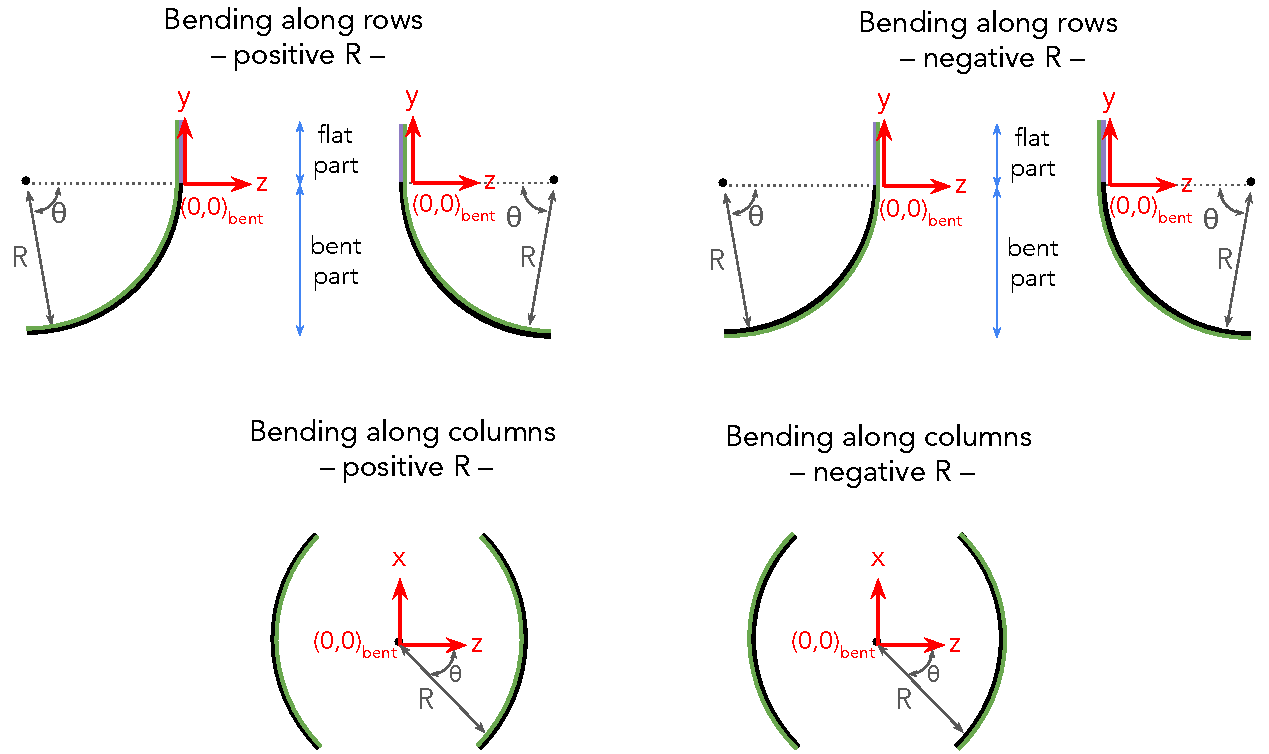
\includegraphics[width=.81\linewidth]{bending_and_radius_definition.pdf}
  \caption{Coordinate system and geometry for sensors bent along the rows or columns. Local bent coordinate system definition (\textcolor{red}{red color}). Bent sensors are depicted with \textbf{black}. Their top side (eg: the part with circuitry for MAPS) is depicted with \textcolor{green}{green}. The convexity/concavity of sensors is defined with respect to the position of their top side (see the parameter \protect\parameter{radius} in Sec.~\ref{sssec:cylindrical_coord_system_params}). \\ Note: a rotation of \SI{180}{\degree} around the $y$-axis (for the sensors bent along rows) or $x$-axis (for sensors bent along the columns) respectively will have the same radius sign. Only the eversion of the sensor will yield a sign change of the radius.}
\label{fig:bent_coord_syst}
\end{figure}


\subsubsection{Cylindrical and cartesian coordinate transformations}
\label{sssec:cylindrical_coord_transformations}

Let ($x$, $y$, $z$) be the standard Cartesian coordinates, and ($r$, $\theta$, $z$) the standard cylindrical coordinates, with $\theta$ the azimuthal angle. The coordinate transformations from cylindrical to cartesian (rectangular) and back, respectively:

\begin{alignat*}{2}
  & \begin{dcases}
  x = \ R \ \text{cos $\theta$}\\
  y = \ R \ \text{sin $\theta$} \\
  z = \ z
  \end{dcases}
    & \hspace{5em} & \begin{dcases}
  \text{sin} \ \theta \ = \cfrac{y}{R}\\
  R \ = \sqrt{x^2+y^2} \\
  z = \ z
  \end{dcases}
\end{alignat*}



\subsubsection{Geometry file settings}
\label{sssec:cylindrical_coord_system_params}

\begin{itemize}
    \item The \parameter{bent_axis} parameter specifies how the sensor is bent (see Fig.~\ref{fig:bent_coord_syst}). Two options are available: \texttt{row} and \texttt{column}. 
    \item The optional \parameter{rotate_by} parameter is used to specify an angle of rotation around the cylinder. Positive values represent a clockwise rotation, as shown in Fig.~\ref{fig:rotated_sensors} for a rotation of half a sensor length clockwise. N.B.: $\theta = \frac{s}{R}$. Defaults to `0deg'.
    \item The \parameter{radius} parameter specifies the bending radius of the sensor. The sign of the radius specifies how the sensor is bent (convex/concave) with respect to its top side (eg: the circuitry part on MAPS): a positive radius is defined for a geometry where the circuitry is decompressed (bent outward), while a negative radius is defined for a sensor with compressed circuitry (bent inward). Examples of the various radius definitions and rotations are given in Fig.~\ref{fig:bent_coord_syst}, Fig.~\ref{fig:rotated_sensors_along_rows}, Fig.~\ref{fig:rotated_sensors_along_col_1} and Fig.~\ref{fig:rotated_sensors_along_col_2}. 
    
    Note that rotations do not change the convexity/concavity, therefore the radius stays as defined (positive or negative). Eversion however will change the radius of the sensors.
    \end{itemize}
    
    
    
    \begin{figure}[!htp]
    \centering
    \begin{subfigure}{.45\textwidth}
      \centering
      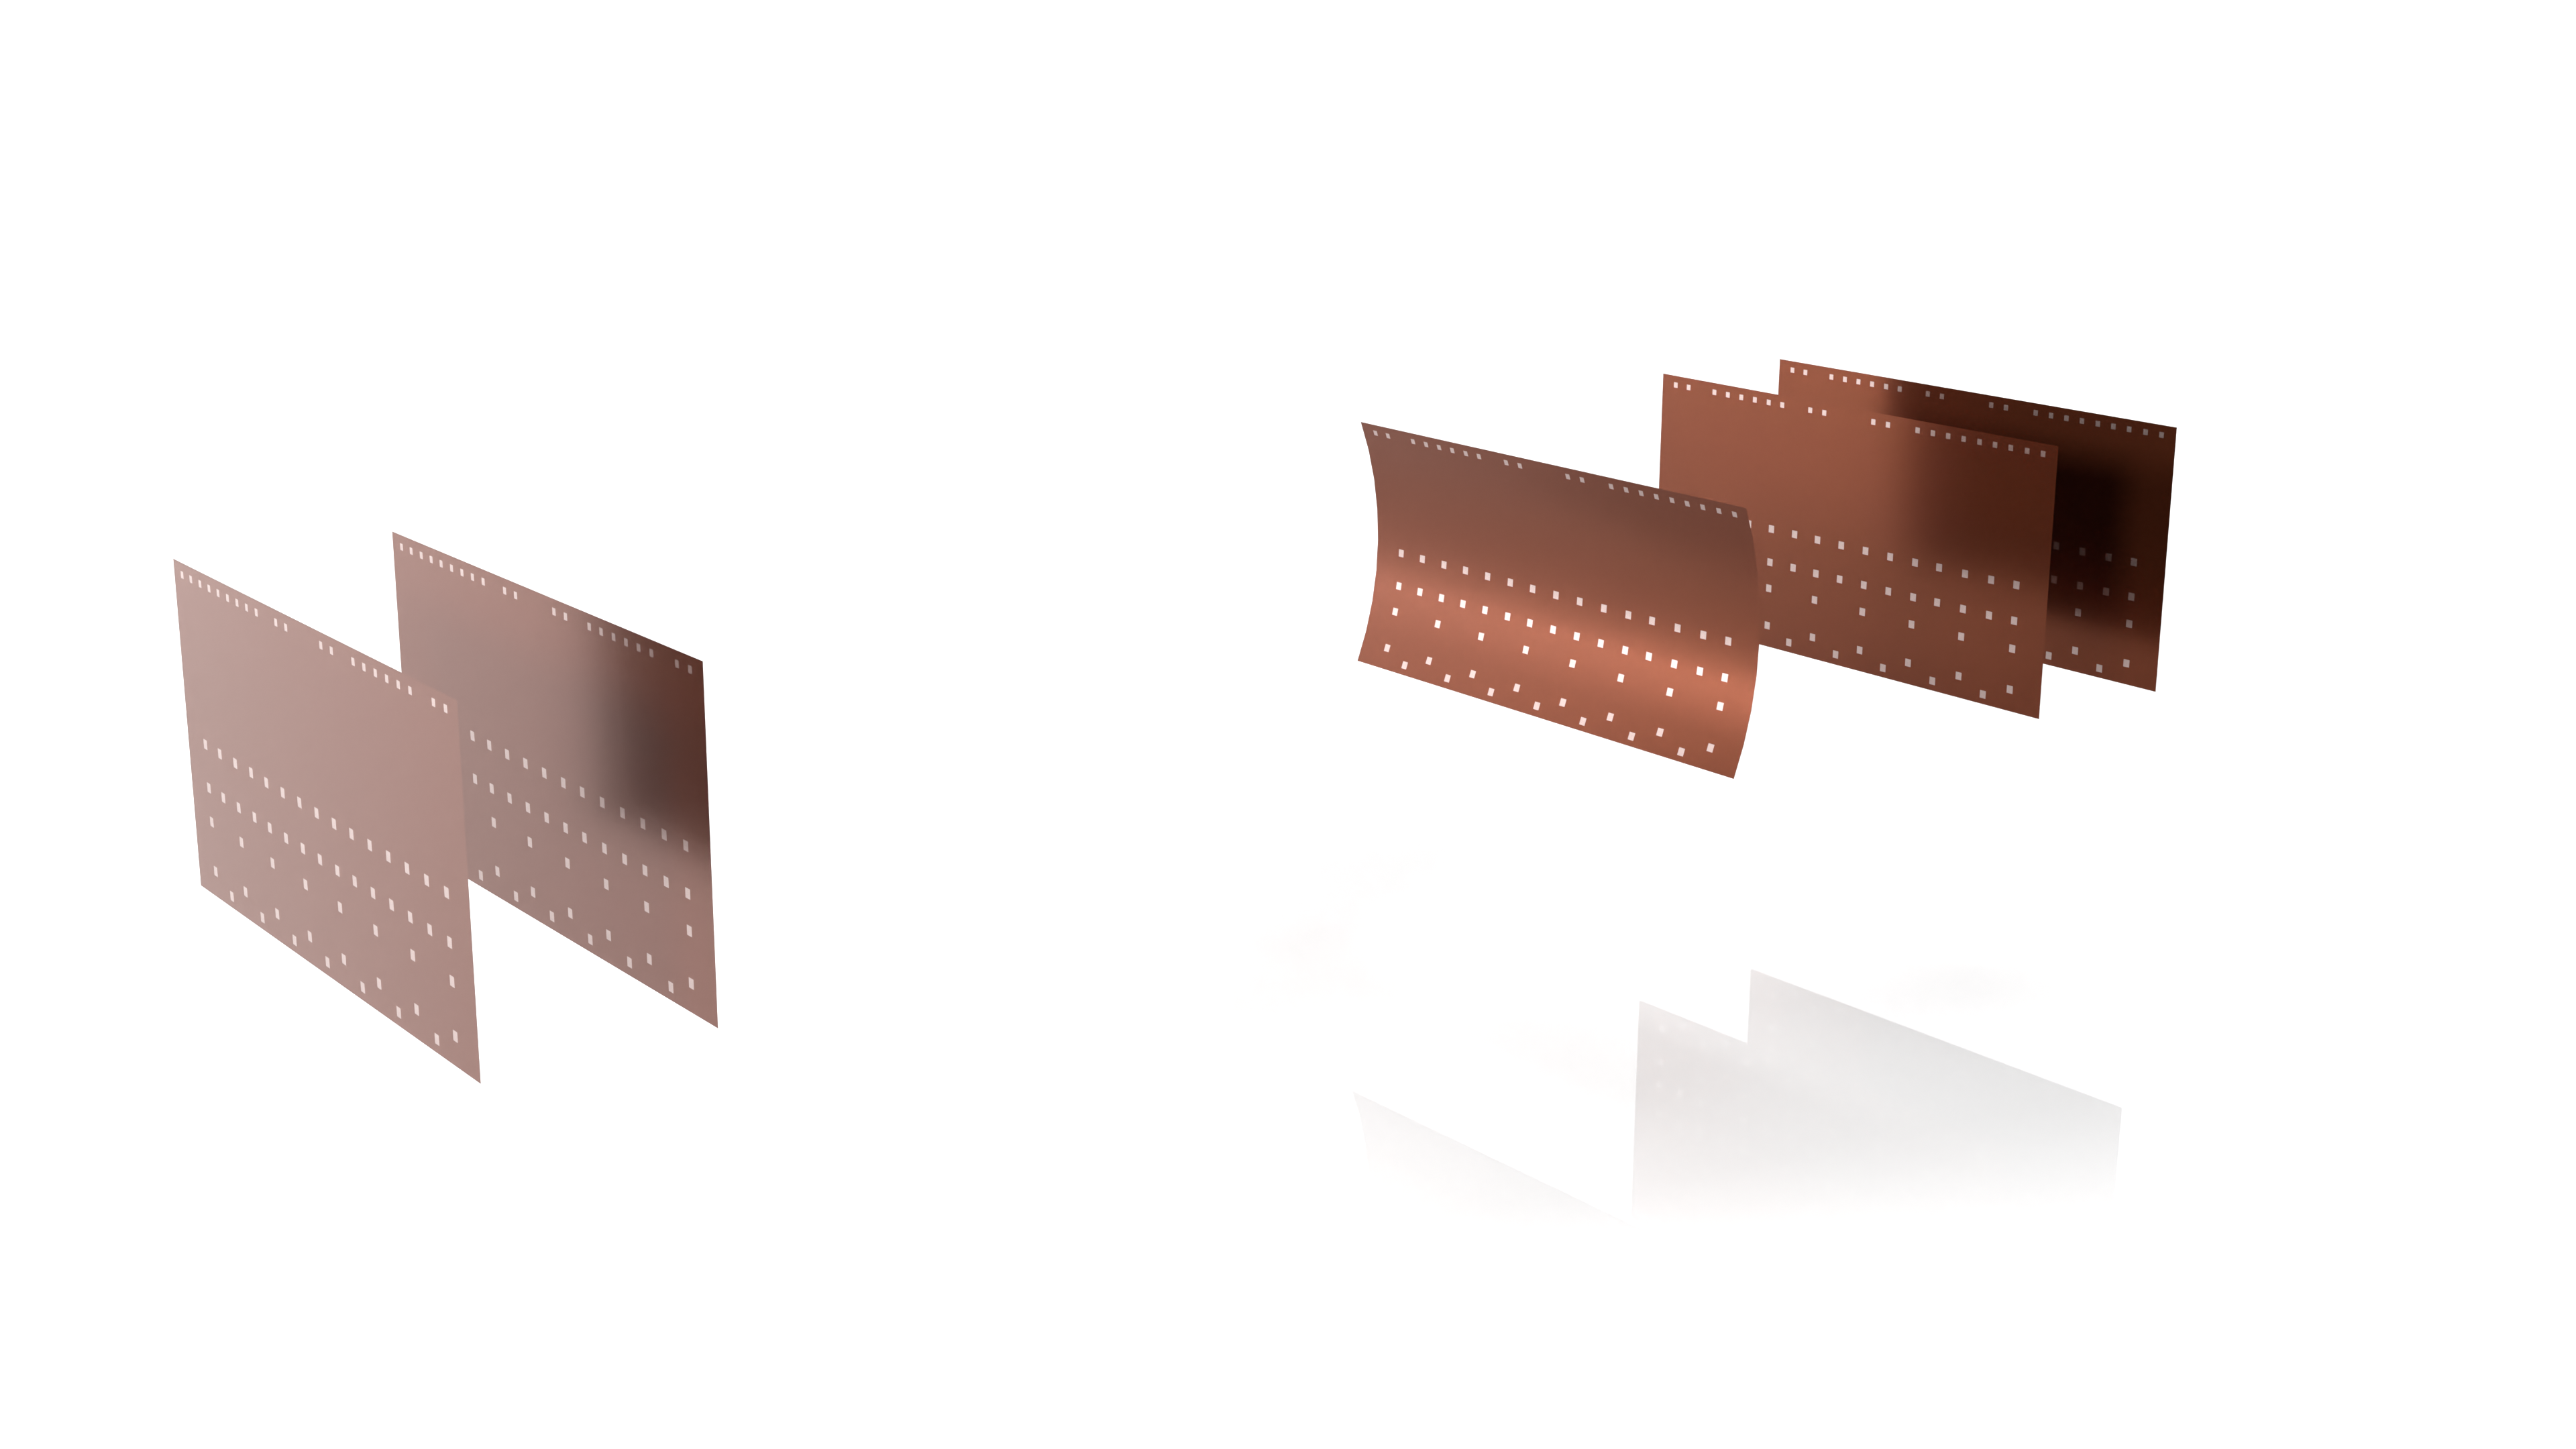
\includegraphics[width=.95\linewidth]{bent_along_rows_1.png}
      \caption{}
      \label{fig:upstream}
    \end{subfigure}%
    \begin{subfigure}{.45\textwidth}
      \centering
      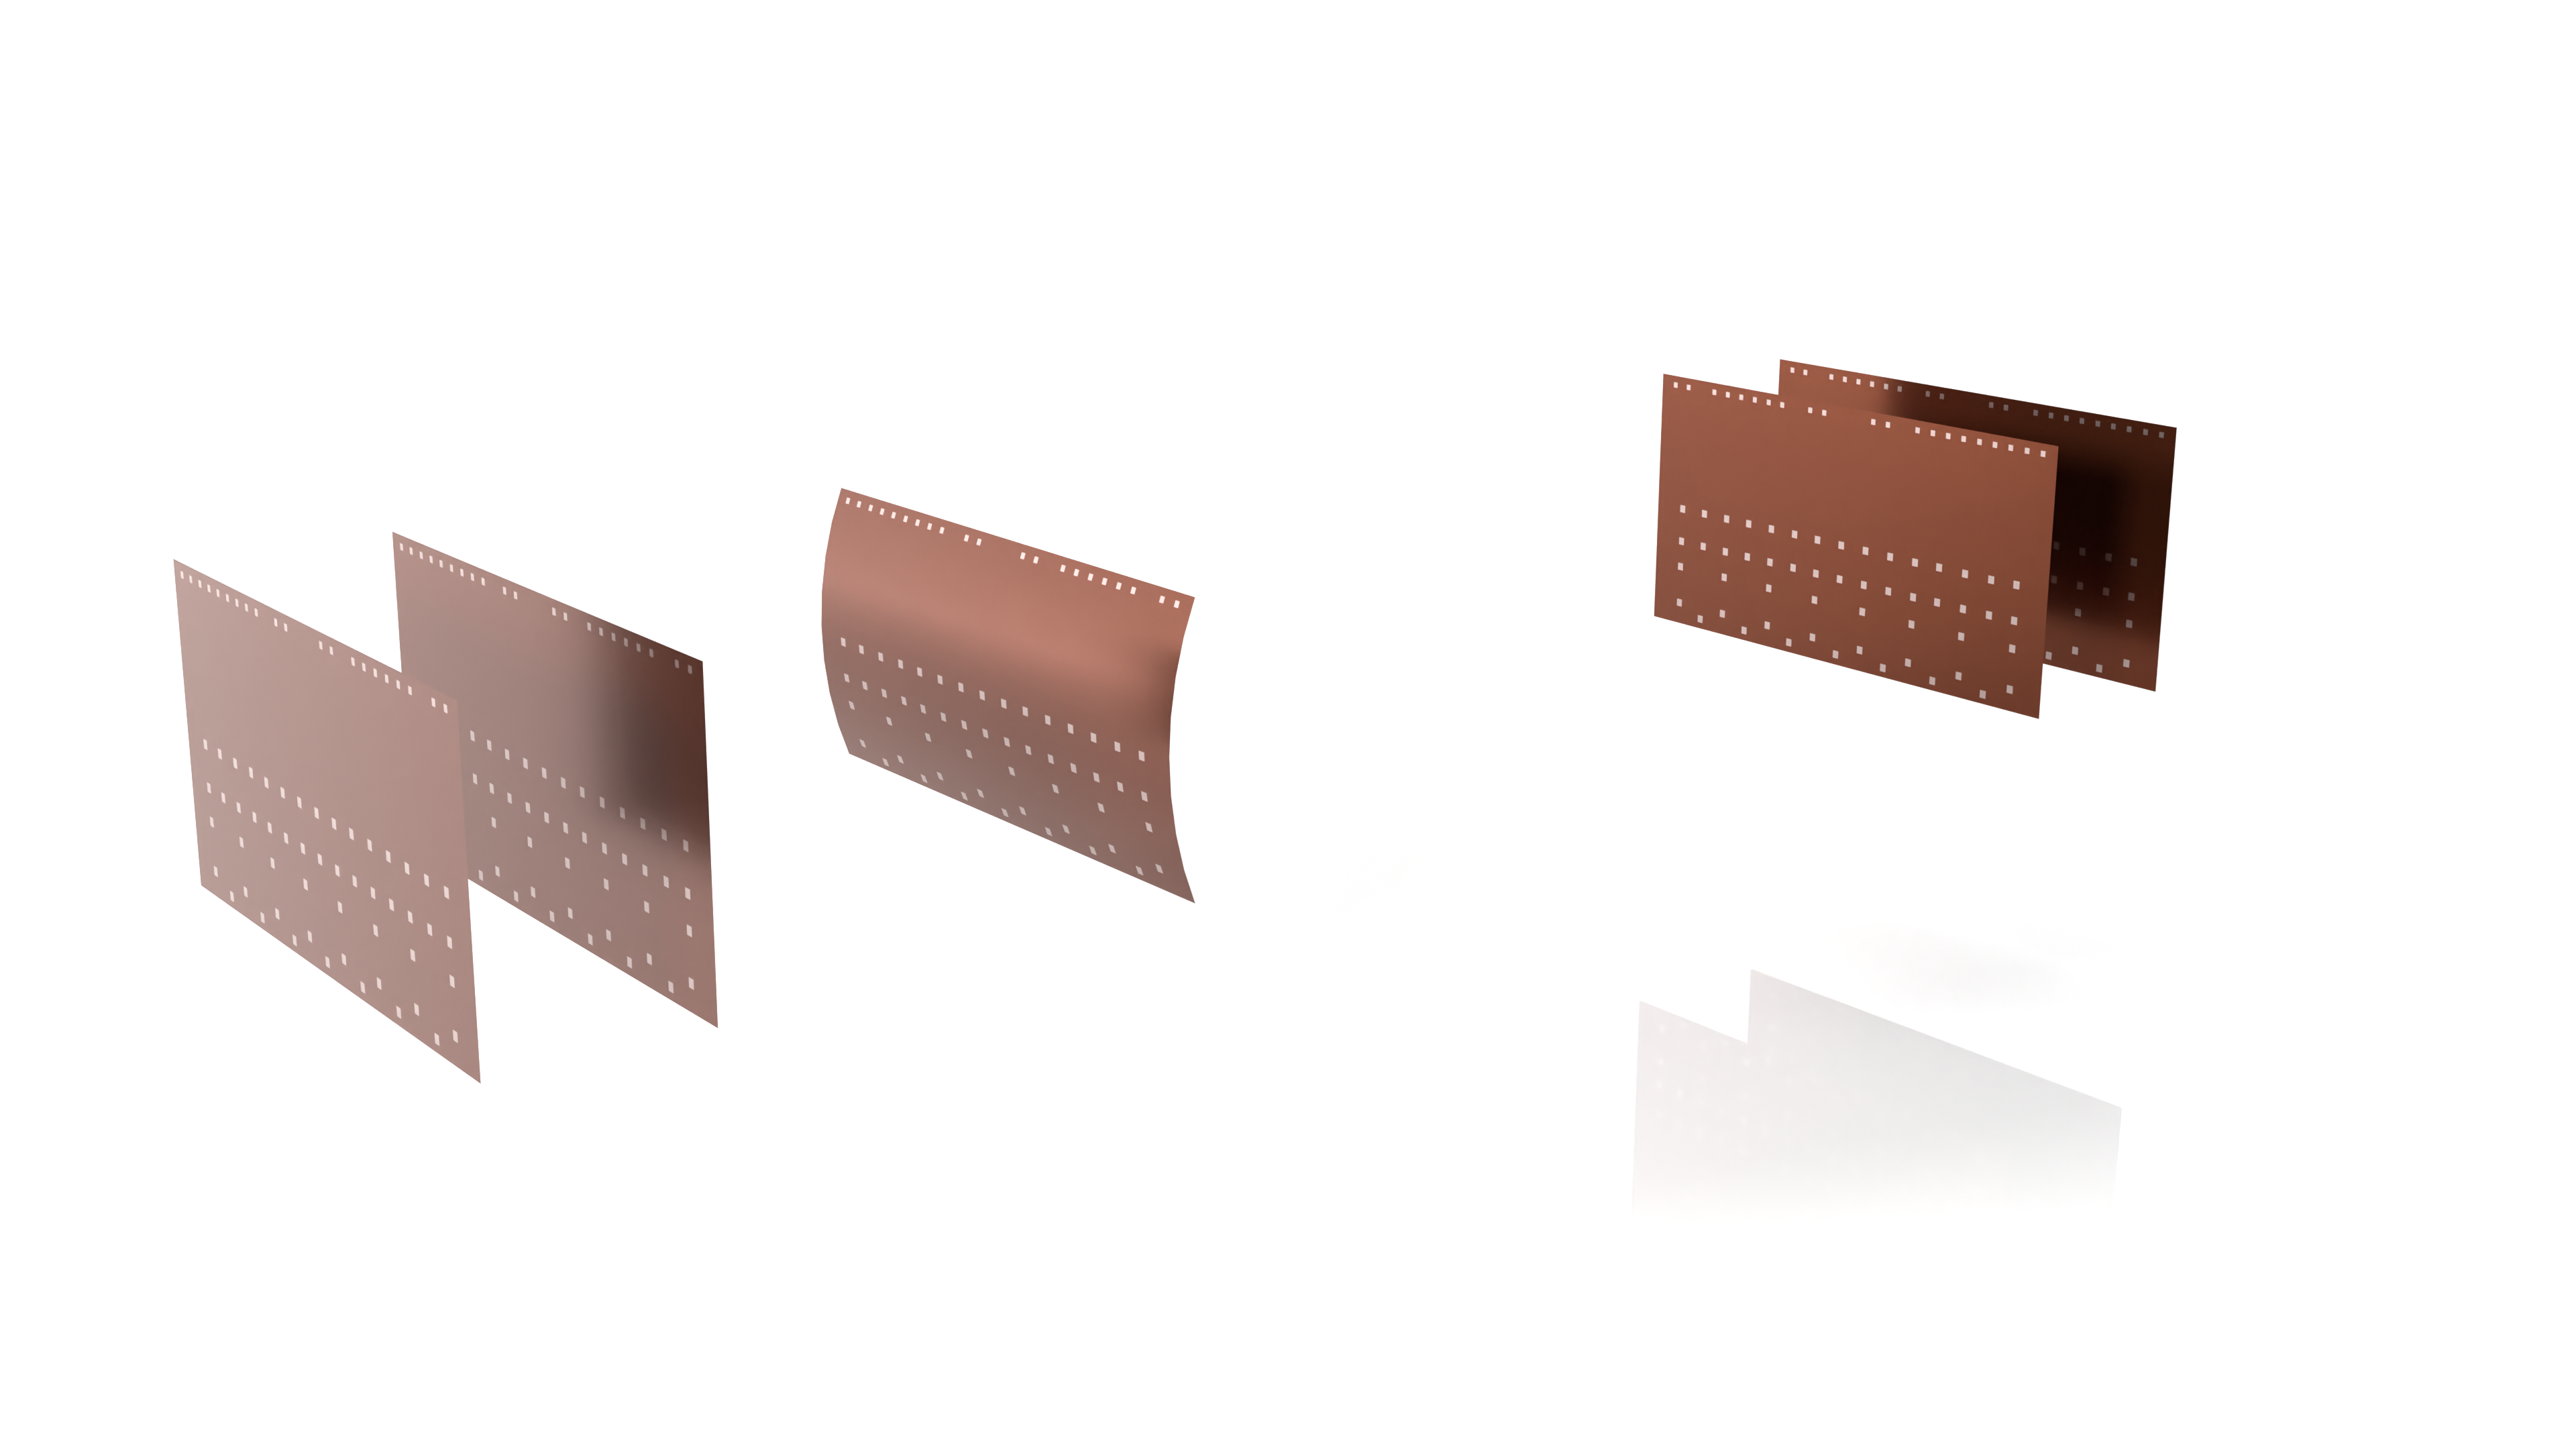
\includegraphics[width=.95\linewidth]{bent_along_rows_2.png}
      \caption{}
      \label{fig:downstream}
    \end{subfigure}
    \begin{multicols}{2}
    \begin{minted}[frame=single,framesep=3pt,breaklines=true,tabsize=2]{ini}
    bent_axis = "row"
    coordinates = "cartesian-bent"
    orientation = 0deg,0deg,0deg
    orientation_mode = "xyz"
    radius = 18mm
    \end{minted}
    \begin{minted}[frame=single,framesep=3pt,breaklines=true,tabsize=2]{ini}
    bent_axis = "row"
    coordinates = "cartesian-bent"
    orientation = 0deg,0deg,0deg
    orientation_mode = "xyz"
    radius = -18mm
    \end{minted}
    \end{multicols}
    \caption{Sensors bent along rows with opposite radius, \protect\parameter{flat_part = 0} and no rotation with respect to the reference chips.}
    \label{fig:rotated_sensors_along_rows}
    \end{figure}
    
    
    
    \begin{figure}[!htp]
    \centering
    \begin{subfigure}{.45\textwidth}
      \centering
      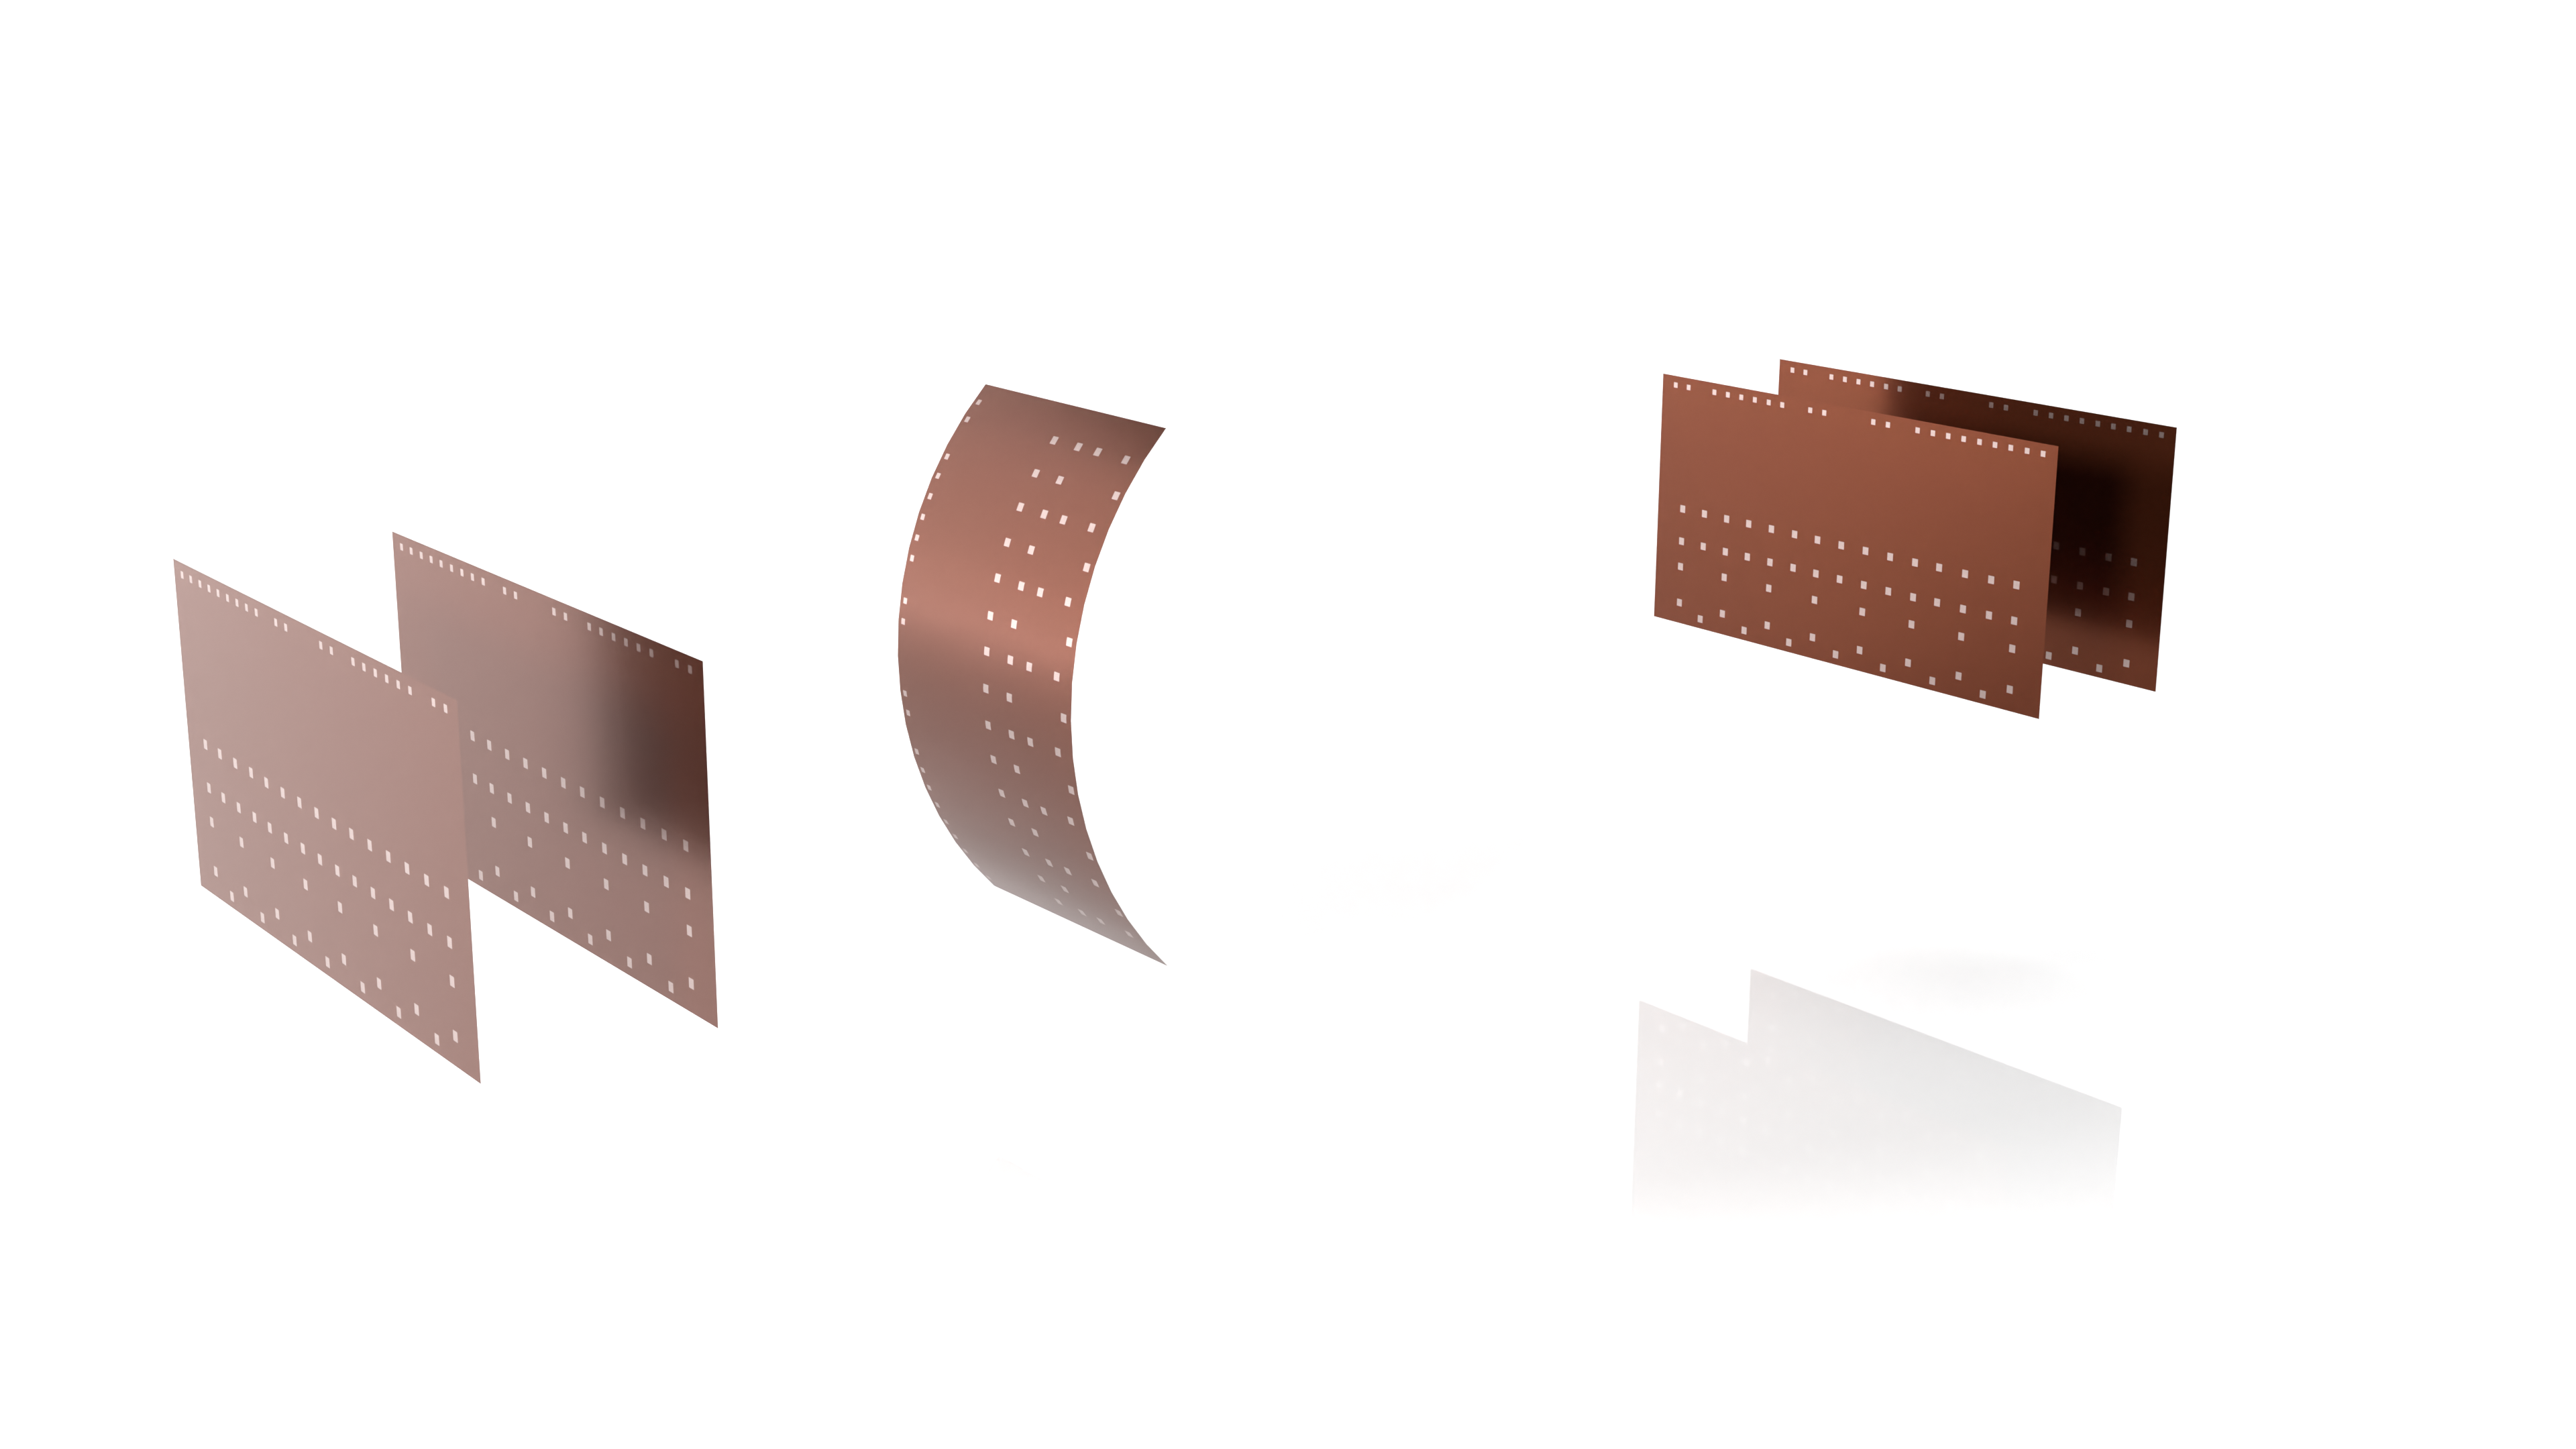
\includegraphics[width=.95\linewidth]{bent_along_cols_1.png}
      \caption{}
      \label{fig:upstream}
    \end{subfigure}%
    \begin{subfigure}{.45\textwidth}
      \centering
      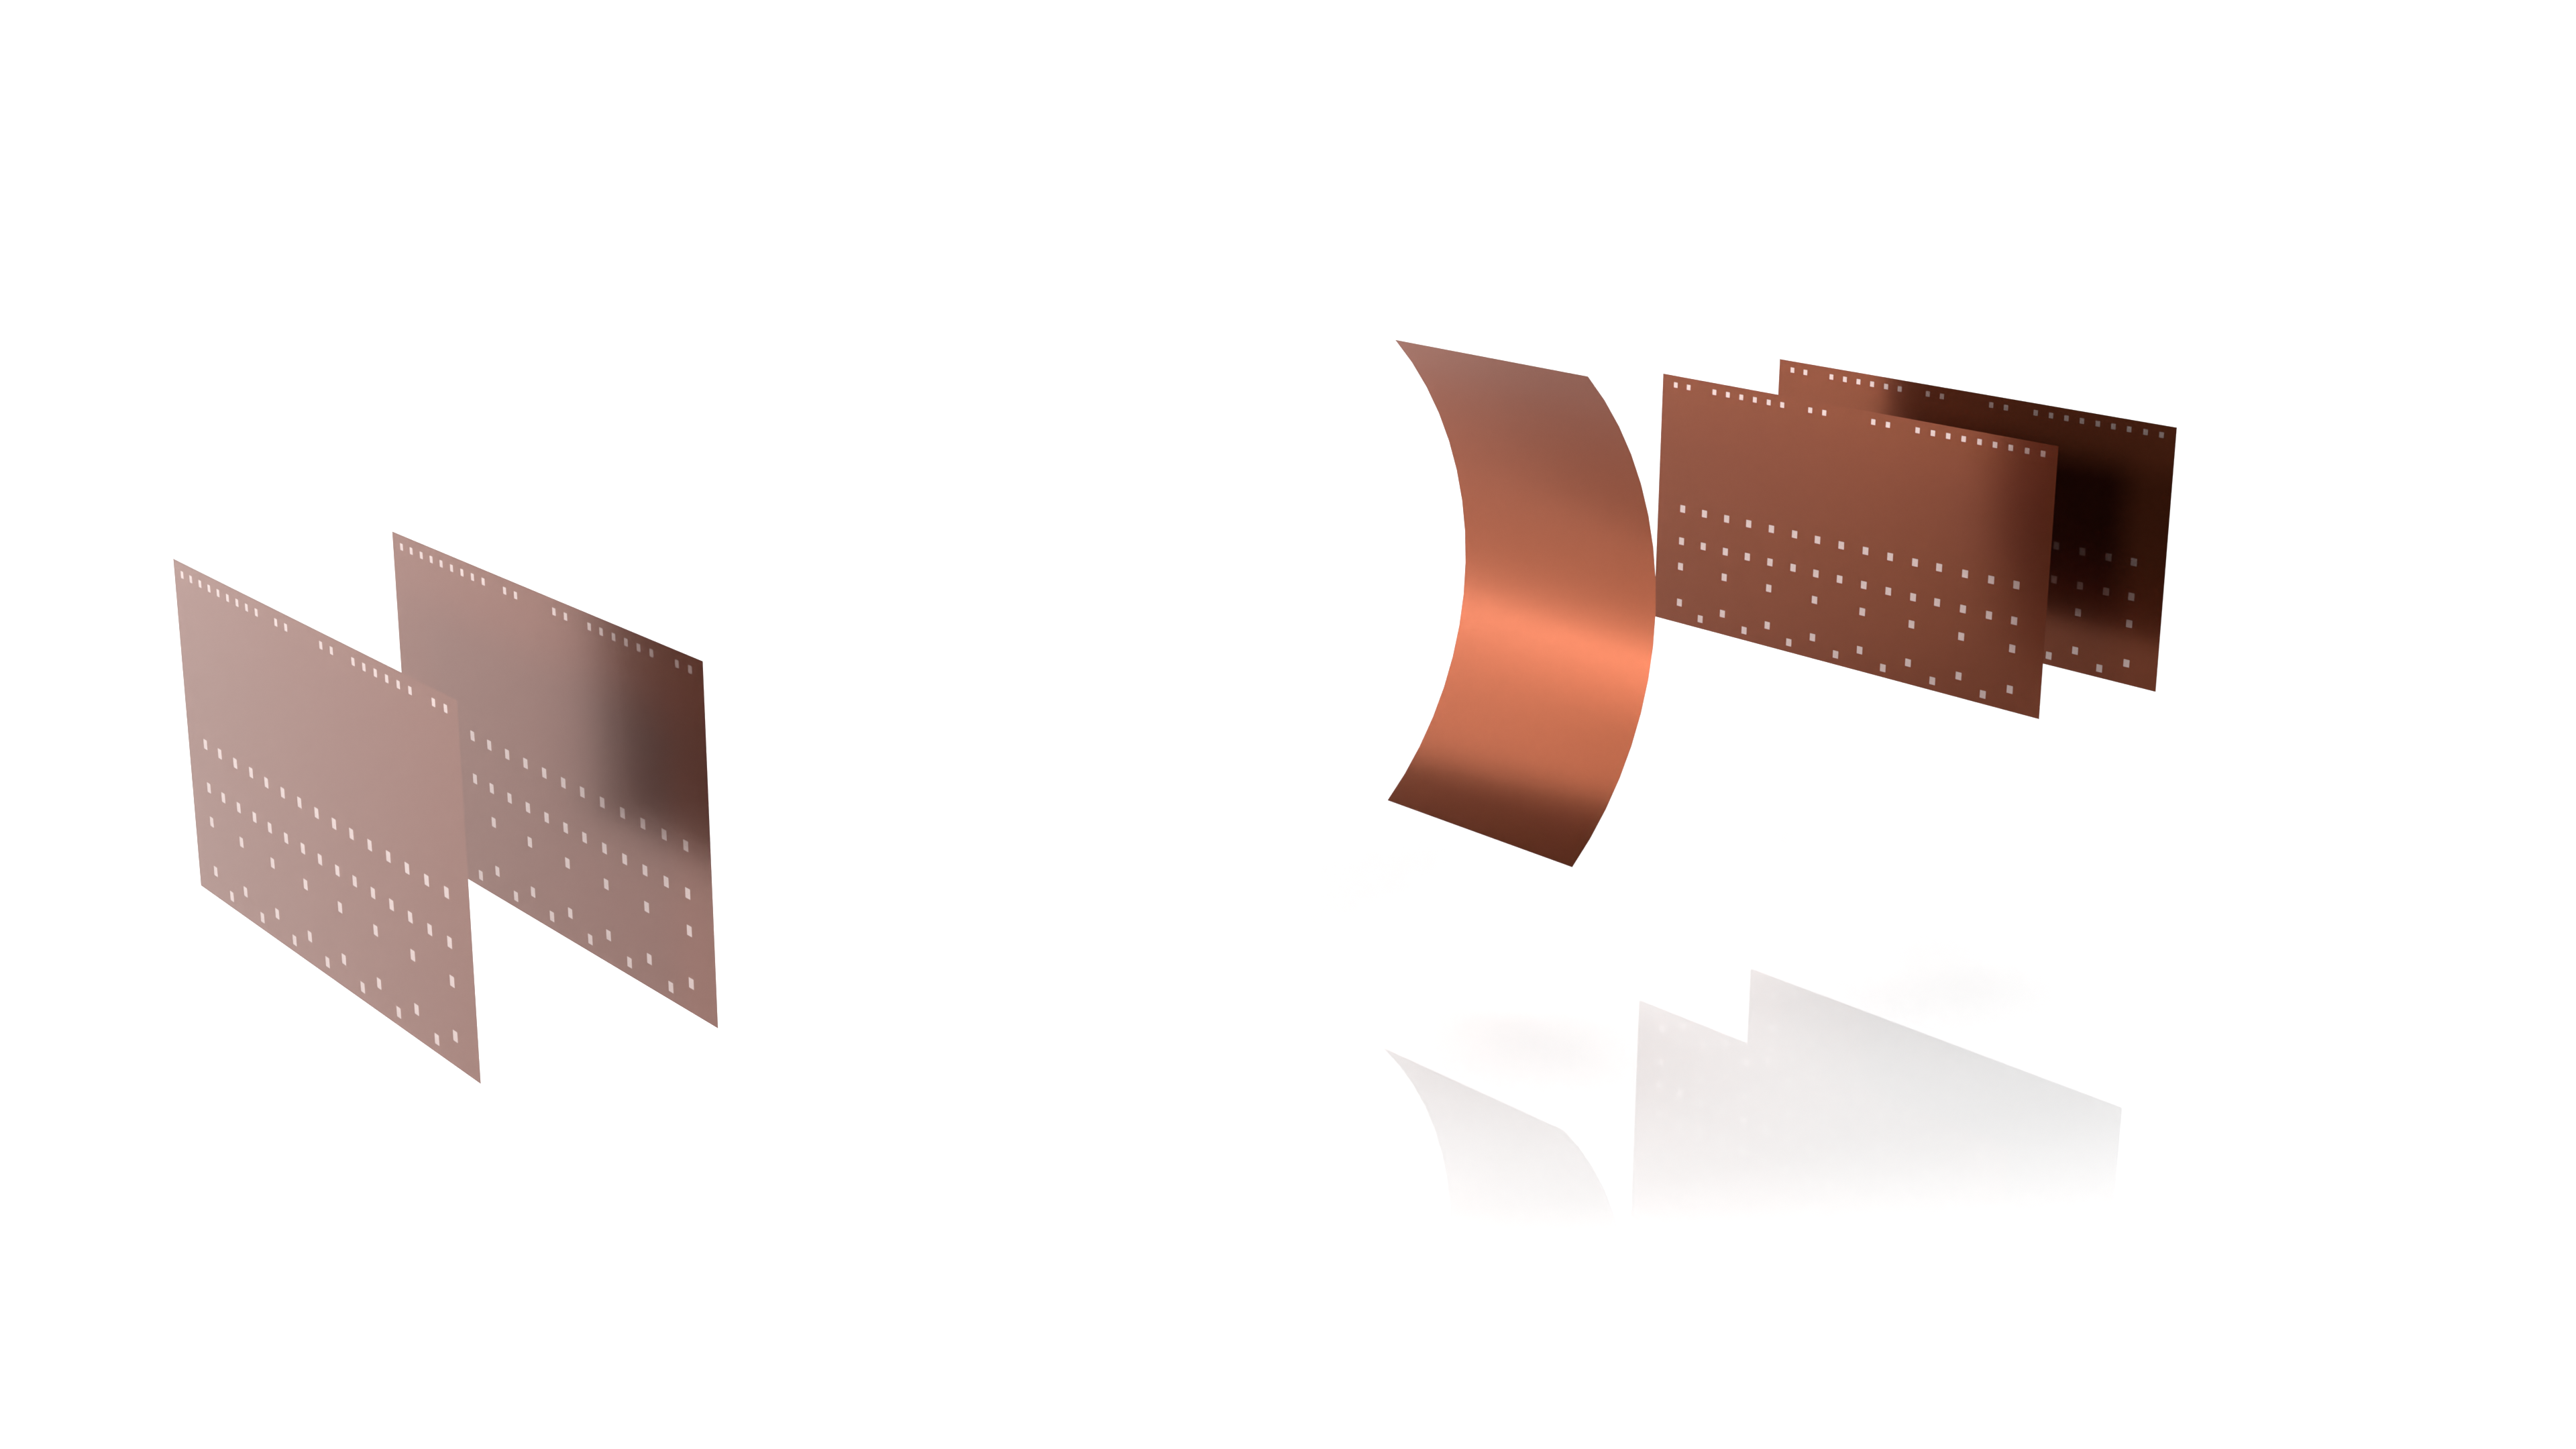
\includegraphics[width=.95\linewidth]{bent_along_cols_2.png}
      \caption{}
      \label{fig:downstream}
    \end{subfigure}
    \begin{multicols}{2}
    \begin{minted}[frame=single,framesep=3pt,breaklines=true,tabsize=2]{ini}
    bent_axis = "column"
    coordinates = "cartesian-bent"
    orientation = 0deg,0deg,90deg
    orientation_mode = "xyz"
    radius = -18mm
    \end{minted}
    \begin{minted}[frame=single,framesep=3pt,breaklines=true,tabsize=2]{ini}
    bent_axis = "column"
    coordinates = "cartesian-bent"
    orientation = 0deg,180deg,90deg
    orientation_mode = "xyz"
    radius = -18mm
    \end{minted}
    \end{multicols}
    \caption{Sensors with the same radius, but rotated by \SI{180}{\degree} with respect to one another. The front side of the sensors is denoted by the pads on the matrix. The device under test (middle sensor) in (b) is seen here from the back.}
    \label{fig:rotated_sensors_along_col_1}
    \end{figure}
    
    
    \begin{figure}[!htp]
    \centering
    \begin{subfigure}{.45\textwidth}
      \centering
      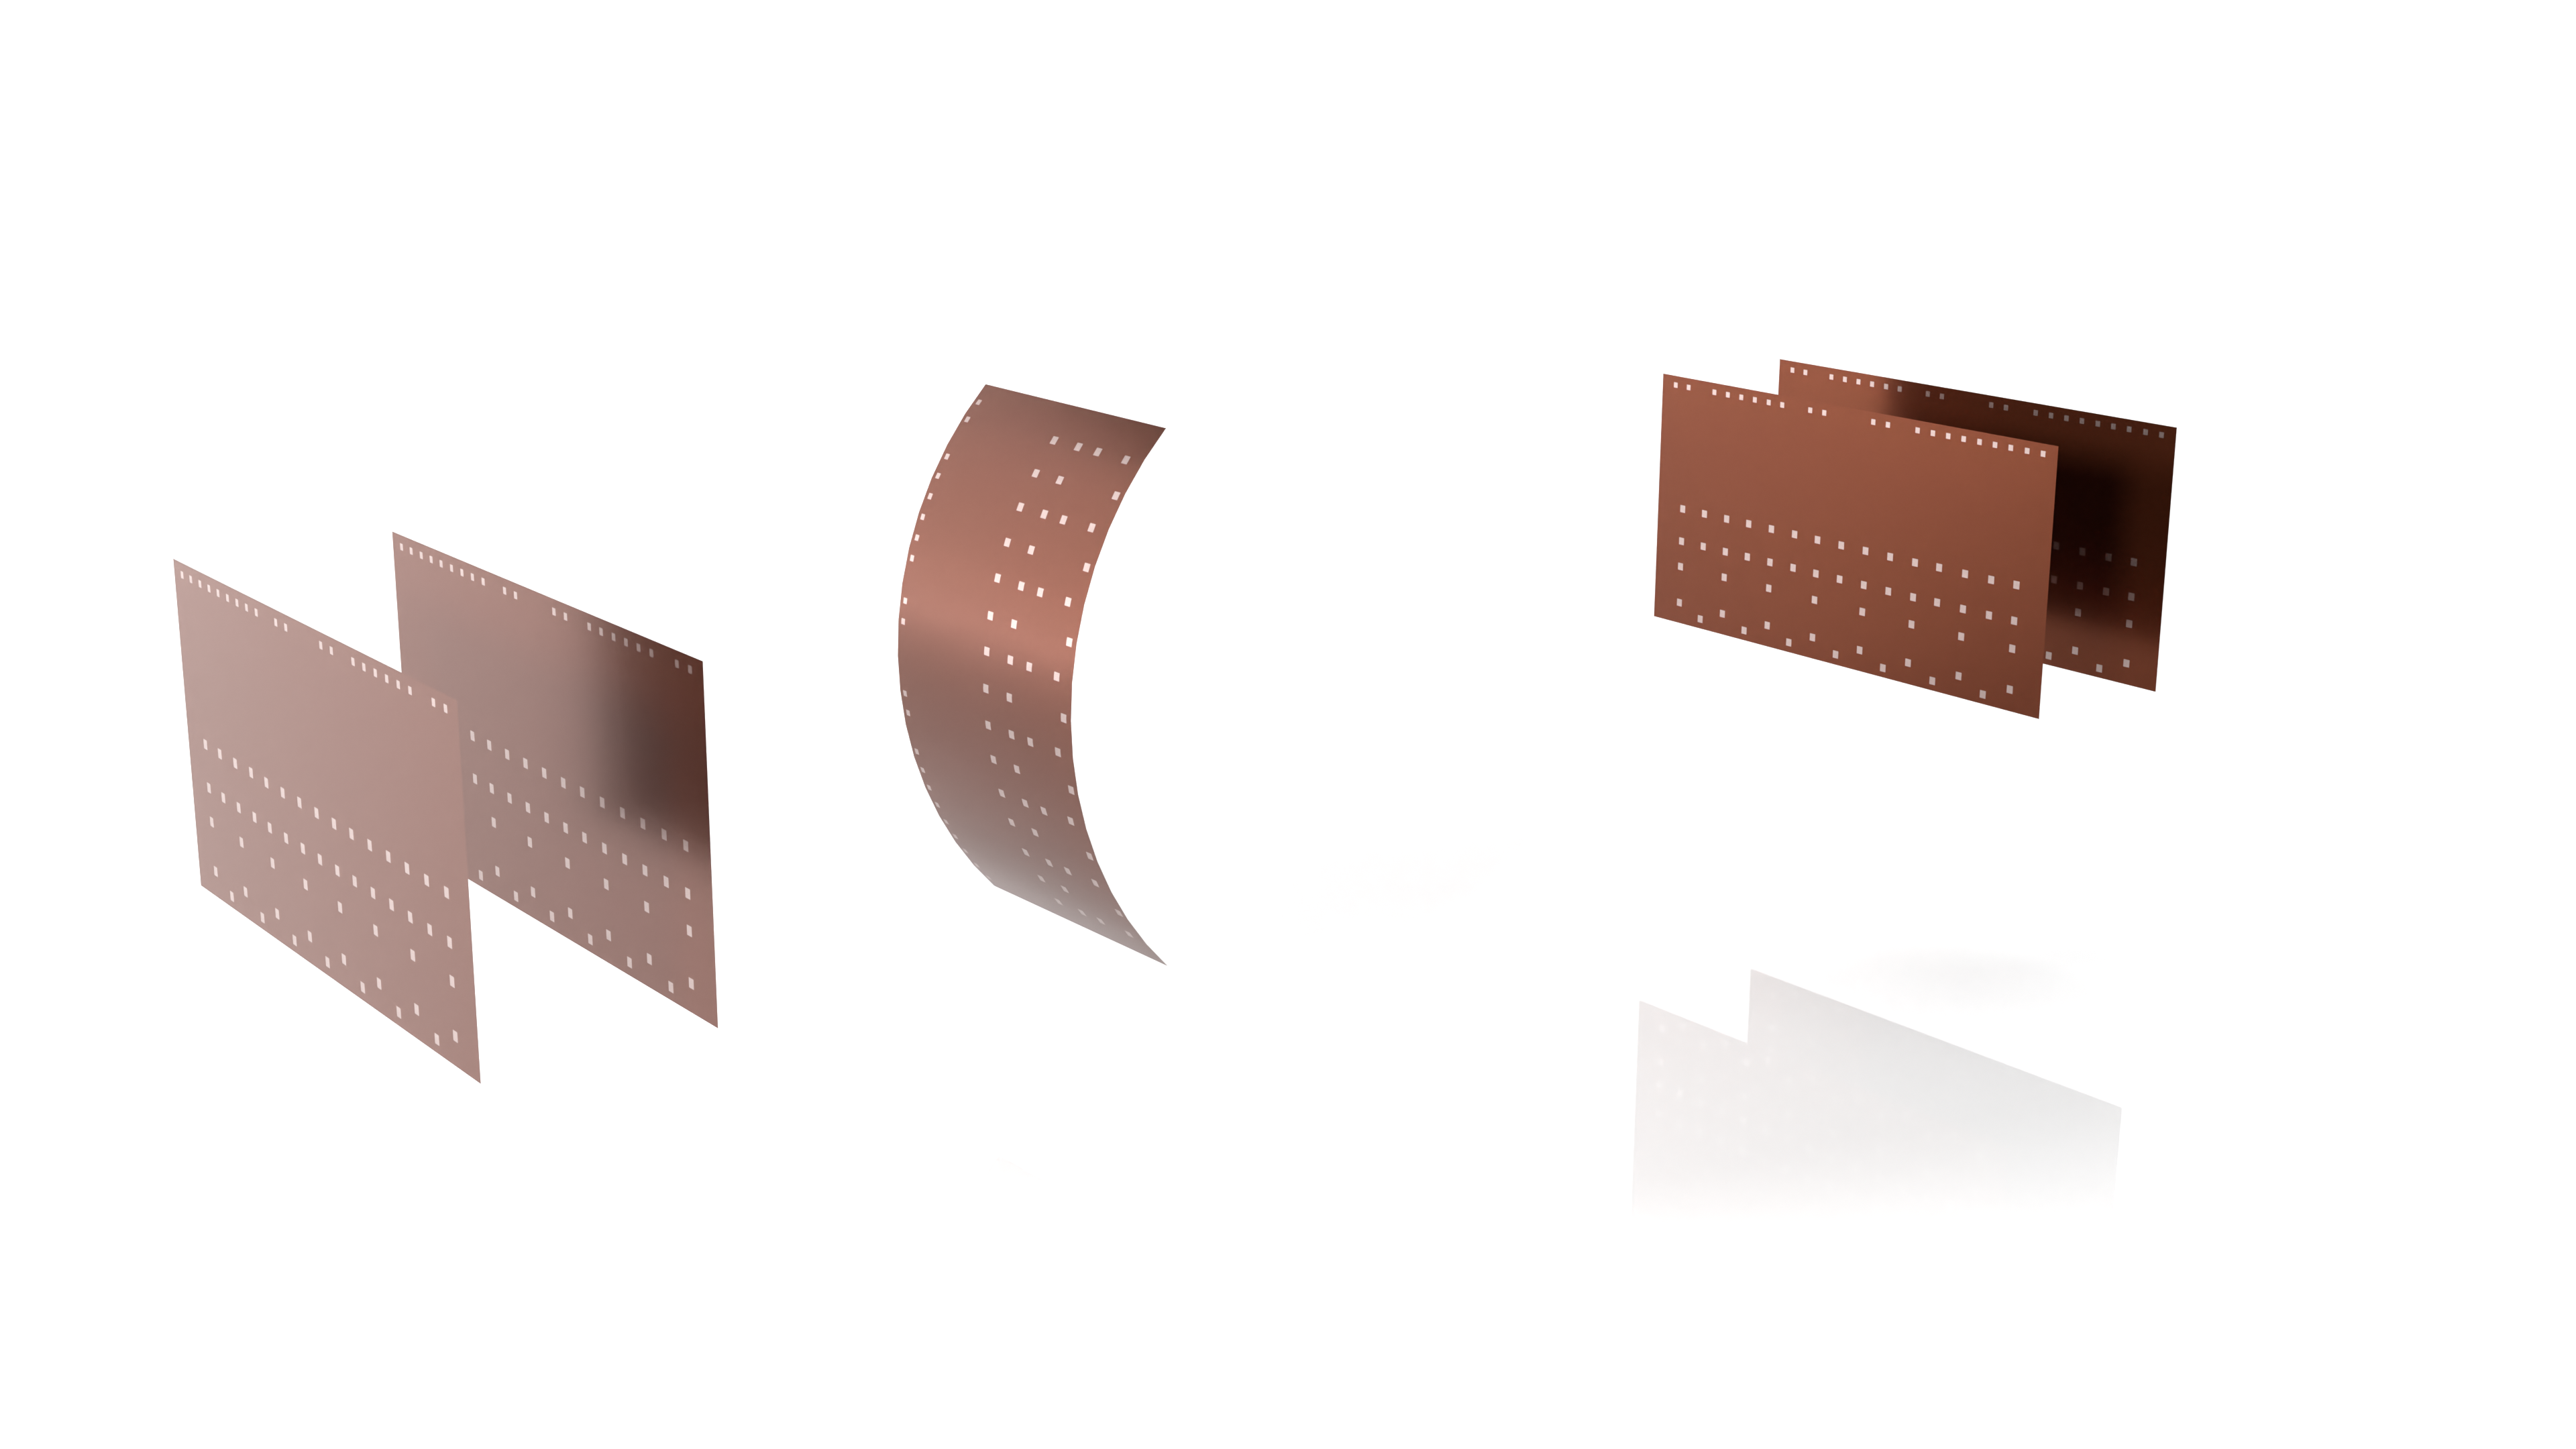
\includegraphics[width=.95\linewidth]{bent_along_cols_1.png}
      \caption{}
      \label{fig:upstream}
    \end{subfigure}%
    \begin{subfigure}{.45\textwidth}
      \centering
      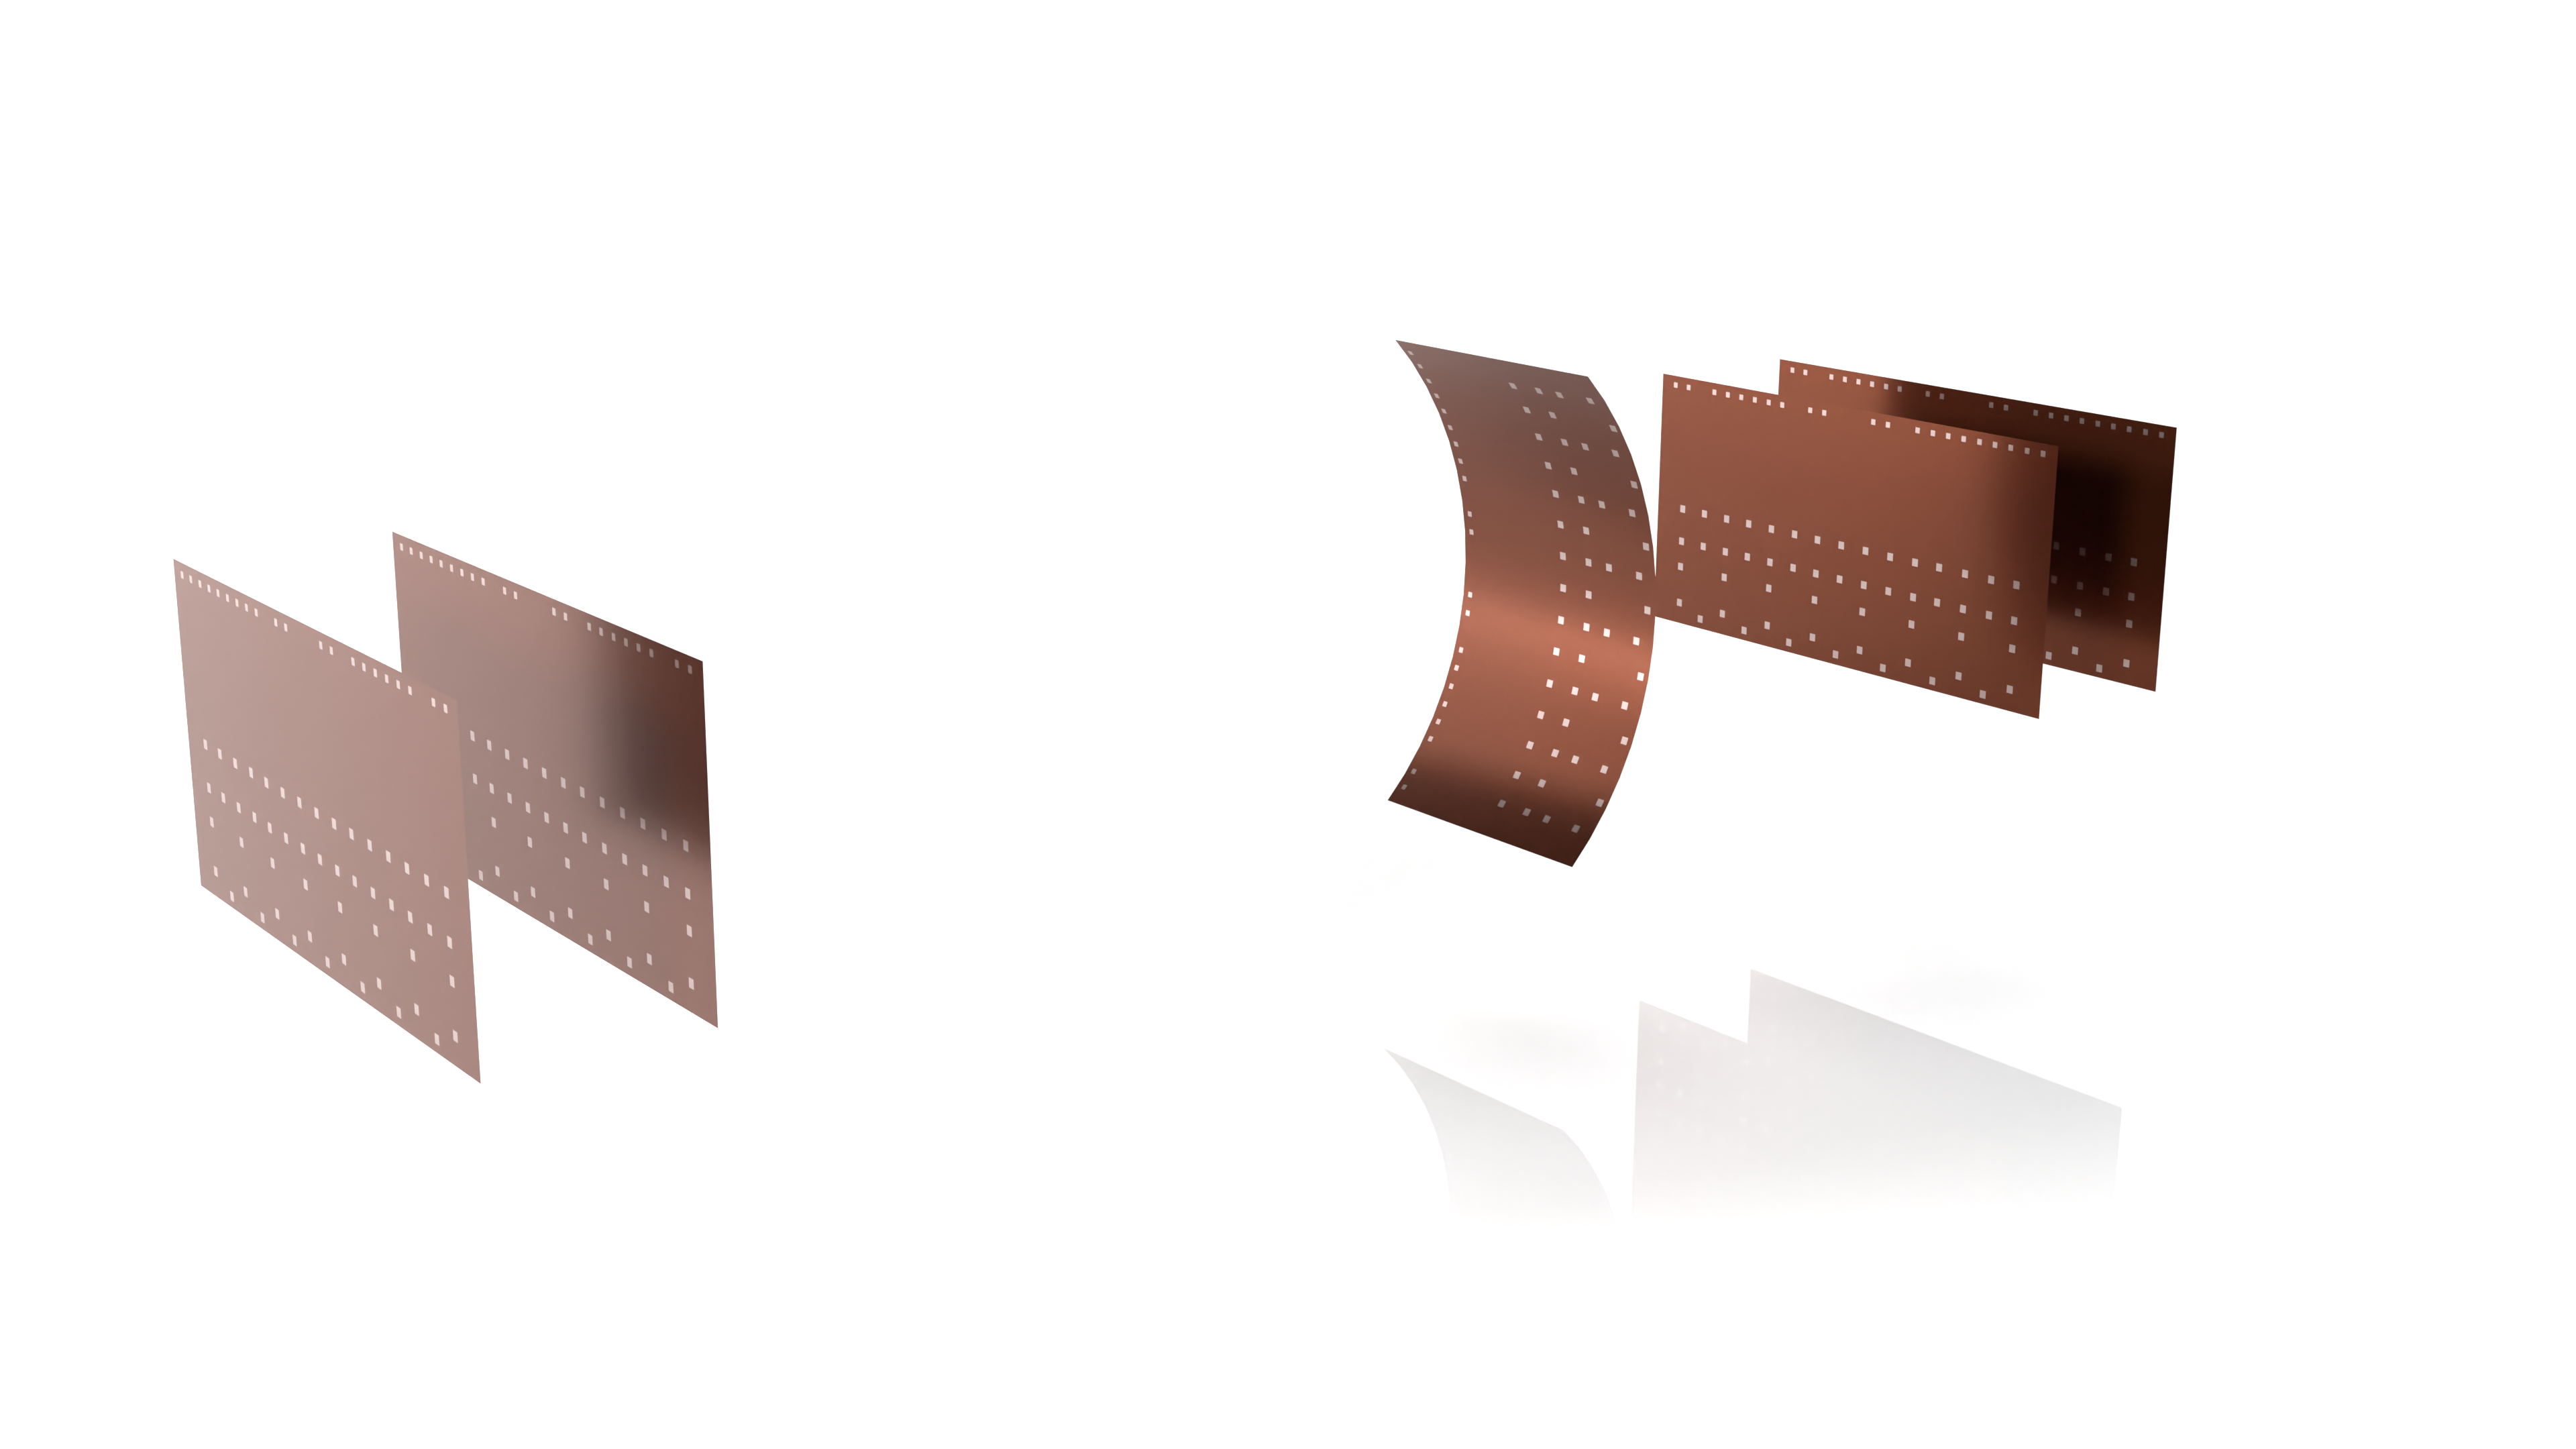
\includegraphics[width=.95\linewidth]{bent_along_cols_3.png}
      \caption{}
      \label{fig:downstream}
    \end{subfigure}
    \begin{multicols}{2}
    \begin{minted}[frame=single,framesep=3pt,breaklines=true,tabsize=2]{ini}
    bent_axis = "column"
    coordinates = "cartesian-bent"
    orientation = 0deg,0deg,90deg
    orientation_mode = "xyz"
    radius = -18mm
    \end{minted}
    \begin{minted}[frame=single,framesep=3pt,breaklines=true,tabsize=2]{ini}
    bent_axis = "column"
    coordinates = "cartesian-bent"
    orientation = 0deg,0deg,90deg
    orientation_mode = "xyz"
    radius = 18mm
    \end{minted}
    \end{multicols}
    \caption{Sensors with opposite radii, rotated only with respect to the reference detectors by \SI{90}{\degree} and not with respect to one another.}
    \label{fig:rotated_sensors_along_col_2}
    \end{figure}